%----------------------------------------------------------------------
\section[Astrodynamics]{Astrodynamics: the two body problem}
%----------------------------------------------------------------------

%----------------------------------------------------------------------
\paragraph{Position, velocity and acceleration of point particle}
%----------------------------------------------------------------------

In Cartesian coordinates, and calling $\bm i,\bm j, \bm k$ the unit vectors
of the basis of our inertial reference frame, the position $\bm r$, velocity 
$\bm v$ and acceleration $\bm a$ vectors of a point particle $P$ are defined 
as:
%
\begin{align}
\bm r &= x\bm i + y \bm j + z \bm k
\\
\bm v &= v_x\bm i + v_y \bm j + v_z \bm k
\\
\bm a &= a_x\bm i + a_y \bm j + a_z \bm k
\end{align}
%
The velocity is the derivative of the position, and the acceleration is the 
derivative of the velocity. Conversely, the position is the integral of the 
velocity, and the velocity is the integral of the acceleration:
%
\begin{align}
\frac{\dd \bm r}{\dd t} &= \bm v;
&\frac{\dd \bm v}{\dd t} &= \bm a;
\\
\bm r &= \int_0^t \bm v \dd t + \bm r_0;
&\bm v &= \int_0^t \bm a \dd t + \bm v_0.
\end{align}
%
Newton's second law of mechanics states that the 
acceleration of a point particle is proportional to the 
sum of all forces acting upon it. The constant of proportionality is its mass:
%
\begin{equation}
m\bm a = \sum \bm F
\end{equation}
%
Thus, knowing the mass and the forces acting on a particle we may compute its 
acceleration. By integrating the acceleration twice we can find how the 
position of the particle changes in time, i.e., its \emph{trajectory}. This
is known as solving the direct problem of mechanics.

%----------------------------------------------------------------------
\paragraph{Newton's law of gravitation}
%----------------------------------------------------------------------

The force exerted upon a point particle of mass $m$ by another of mass $M$ 
located at the origin of coordinates is
%
\begin{equation}
\bm F = - G \frac{mM}{r^2} \bm u_r
\end{equation}
%
where $\bm u_r = \bm r/r$ is the unit vector in the direction of $\bm r$, and
$G=6.67408\cdot 10^{-11}$ m$^3$kg$^{-1}$s$^{-2}$ is the universal 
gravitational constant.

The equation of motion of a point particle in the gravity field of a planet is
then:
%
\begin{equation}
\bm a = \frac{\dd \bm v}{\dd t} = \frac{\dd^2 \bm r}{\dd t^2} = - G\frac{M}{r^2}\bm u_r
\label{eq:motion}
\end{equation}

%----------------------------------------------------------------------
\paragraph{Conservation of mechanical energy}
%----------------------------------------------------------------------

The mechanical energy of a point particle in the gravity field of a planet 
like the Earth is $E = E_{kin}+E_{pot}$, where 
%
\begin{equation}
E_{kin}=\frac{1}{2}mv^2; \quad E_{pot} = -\frac{GmM}{r}.
\end{equation}
%
The mechanical energy $E$ is a conserved quantity of motion. 

\emph{Demonstration}: by denoting with $\cdot$ the scalar product,
we dot-multiply Eq.~\eqref{eq:motion} by $m\bm v$:
%
\begin{align}
&m\frac{\dd \bm v}{\dd t} \cdot \bm v 
= - G\frac{mM}{r^2}\left(\frac{\bm r}{r}\right) \cdot \bm v
\Rightarrow
\frac{1}{2}m\frac{\dd v^2}{\dd t}
= - G\frac{mM}{r^3}\bm r \cdot \frac{\dd \bm r}{\dd t} 
= - G\frac{mM}{2r^3}\frac{\dd r^2}{\dd t} 
= GmM\frac{\dd }{\dd t} \left(\frac{1}{r}\right)
\\
&\frac{\dd }{\dd t} \left(\frac{1}{2}mv^2 -\frac{GmM}{r}\right) = 0
\Rightarrow
\frac{1}{2}mv^2 -\frac{GmM}{r} = E = \const.
\end{align}

%----------------------------------------------------------------------
\paragraph{Conservation of angular momentum}
%----------------------------------------------------------------------

The angular momentum of a point particle about the origin is defined as
%
\begin{equation}
\bm H = m\bm r \times \bm v,
\end{equation}
%
where $\times$ is the vector product. $\bm H$ is a vector that is conserved in 
the motion. Its magnitude can be written as $H=mr^2 \dd \theta/\dd t$, where 
$\theta$ is the polar angle of the motion of the particle.

\emph{Demonstration}: we cross-multiply Eq.~\eqref{eq:motion} by $m\bm r$. The 
right-hand-side is identically zero thanks to the properties of the vector 
product:
%
\begin{equation}
m\bm r\times \bm a
= - G\frac{mM}{r^2}\bm r\times \left(\frac{\bm r}{r}\right) = 0.
\end{equation}
%
We now apply the following identity
%
\begin{equation}
\frac{\dd}{\dd t}\left(m\bm r \times \bm v\right) 
= m \bm v \times \bm v + m\bm r \times \bm a =  m\bm r \times \bm a,
\end{equation}
%
and conclude that
%
\begin{equation}
\frac{\dd \bm H}{\dd t} = 0 \Rightarrow \bm H = \const.
\end{equation}

%----------------------------------------------------------------------
\paragraph{Conic sections}
%----------------------------------------------------------------------

The trajectory of a point particle in the two body problem of astrodynamics
is a conic section. Conic sections are characterized by their semi-major axis 
$a$ and their eccentricity $e$. The conic section can be any of the following:
%
\begin{enumerate}
\item Ellipse ($a>0$ and $e<1$). The only closed orbit. When $e=0$, the 
ellipse is a circle.
\item Parabola ($a\to \infty$ and $e=1$). A particle in a parabolic trajectory 
will reach infinity with zero velocity. The semi-latus rectum $p=a(1-e^2)$ 
is used instead of $a$ in this case to avoid the indetermination.
\item Hyperbola ($a<0$ and $e>1$). A particle in a parabolic trajectory 
will reach infinity with non-zero velocity. Of the two branches of the 
hyperbola, the trajectory is only one of them.
\end{enumerate}
% 

%----------------------------------------------------------------------
\begin{center}
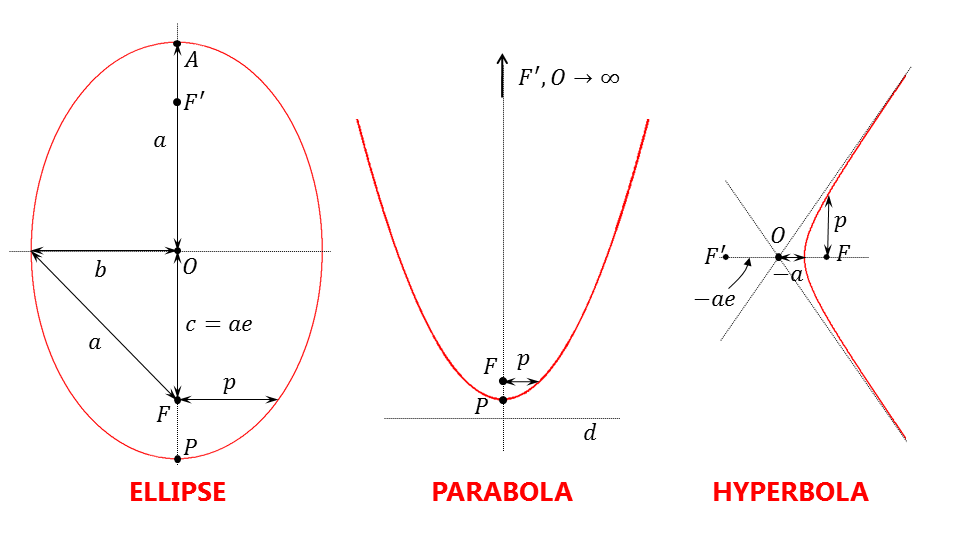
\includegraphics[width=\textwidth]{figs/conics.png}
\end{center}
%----------------------------------------------------------------------

The pericenter and the apocenter are the points of 
the trajectory nearest and farthest away from the planet:
%
\begin{equation}
r_p = a(1-e);\quad r_a = a(1+e).
\end{equation}
%
Observe that the definition of the apocenter only makes sense for elliptic 
orbits. Also, in the case of parabolic orbits, the pericenter can be computed 
simply as $r_p = p/2$.

At the pericenter and apocenter the position and velocity vectors are 
perpendicular to each other, i.e., $\bm r \cdot \bm v = 0$.

%----------------------------------------------------------------------
\paragraph{Vis-viva equation}
%----------------------------------------------------------------------

The constant $E$ in the energy equation is related to the semi-major axis of 
the orbit:
%
\begin{equation}
\frac{1}{2}mv^2 -\frac{GmM}{r} = -\frac{GmM}{2a}
\end{equation}
%

\emph{Demonstration}: 
We particularize the mechanical energy equation at the pericenter and 
the apocenter and subtract the two expressions:
%
\begin{equation}
\frac{1}{2}mv_p^2 -\frac{GmM}{r_p} = E; \quad
\frac{1}{2}mv_a^2 -\frac{GmM}{r_a} = E.
\label{eq:Eparticularized}
\end{equation}
%
\begin{equation}
\frac{1}{2}m\left(v_p^2-v_a^2\right) -GmM\left(\frac{1}{r_p}
-\frac{1}{r_a}\right) = 0;
\label{eq:visvivapartial}
\end{equation}
%
From the conservation of angular momentum, using $2a=r_a+r_p$, 
and since the position and velocity 
vectors are perpendicular at the pericenter and apocenter,
%
\begin{equation}
v_a= \frac{r_p}{2a-r_p}v_p
\end{equation}
%
Substituting $v_a$ in Eq.~\eqref{eq:visvivapartial}, and using again
$2a=r_a+r_p$,
%
\begin{equation}
\frac{1}{2}mv_p^2\left(1-\frac{r_p^2}{(2a-r_p)^2}\right) =
GmM\left(\frac{1}{r_p} -\frac{1}{2a-r_p}\right)
\Rightarrow 
v^2_p=\frac{GM}{a}\left(\frac{2a}{r_p}-1\right) 
\end{equation}
%
Finally, substituting in the first of Eqs.~\eqref{eq:Eparticularized} we 
find $E = -GmM/(2a)$.

Clearly, 
%
\begin{enumerate}
\item Particles in elliptic orbits have negative mechanical energy. The orbit 
is bounded (under no condition could the particle have $r>2a$, as the velocity 
would become imaginary; in reality, the maximum $r$ occurs at apocenter, 
$r_a=a(1-e)$).
\item Particles in parabolic orbits have zero mechanical energy, as they reach 
zero velocity as $r\to \infty$.
\item Particles in hyperbolic orbits have positive mechanical energy, as they 
have a non-zero excess velocity at infinity.
\end{enumerate}

%----------------------------------------------------------------------
\paragraph{Important velocities}
%----------------------------------------------------------------------

There are several important velocity quantities in the two body problem. 
Importantly, these velocities do not depend on the mass of the point particle, 
only on the mass of the planet $M$ and the universal gravitational constant 
$G$:
%
\begin{itemize}
\item Circular velocity: $v_c=\sqrt{GM/r}$. This is the magnitude of the 
velocity that a particle must have at a radius $r$ to be in circular orbit. 
Obtained from vis-viva equation, by imposing that the trajectory is a circle, 
$r=a$. 
\item Escape velocity: $v_e=\sqrt{2GM/r}$. Any particle with this velocity at 
a distance $r$ from the origin is in parabolic orbit, and will reach infinity
with zero velocity. Obtained from vis-viva equation by setting $a=\infty$.
\item Velocity at pericenter, $v_p=\sqrt{GM\frac{1+e}{1-e}}$. Obtained from 
vis-viva equation, particularizing at $r_p=a(1-e)$.
\item Velocity at apocenter, $v_a=\sqrt{GM\frac{1-e}{1+e}}$. Obtained from 
vis-viva equation, particularizing at $r_a=a(1+e)$. Observe that $v_p>v_a$ 
always.
\end{itemize}
%

%----------------------------------------------------------------------
\paragraph{Kepler laws}
%----------------------------------------------------------------------

Johannes Kepler stated his famous three laws of planetary motion before
Newton established his mathematical theory of gravitation and motion:
%
\begin{enumerate}

\item \emph{The orbit of a planet is  an ellipse with the Sun at one focus}.
We now know that, in general, according to the laws of motion and gravitation
of Newton, the trajectory of a point particle (a planet) about the Sun can be
an ellipse, a parabola, or a hyperbola (i.e. any conic section).
    
\item \emph{The vector from the Sun to the planet sweeps out equal areas
during equal intervals of time}. The area sweep rate is $\dd A /\dd t =
(1/2)r^2 \dd\theta /\dd t = H/(2m)$, so this law is a direct consequence of
the conservation of angular momentum.

\item \emph{The square of the orbital period of the planet is proportional to
the cube of the semi-major axis of its ellipse, i.e. $T^2 \propto a^3$}. This
can easily be proven with the explanation above, taking into account that the
area of an ellipse is $A=\pi a b$, where $b=a\sqrt{1-e^2}$ is the semi-minor
axis.

\end{enumerate}





